% Trabalho Prático - Processamento e Análise de Imagens - PUC Minas (Prof. Alexei Machado)
% Grupo Gnn (PREENCHER)
% Componentes (nome - matrícula - curso - campus): PREENCHER os quatro
%   Bernardo PREENCHER - PREENCHER - Ciência da Computação - PREENCHER
%   Diego    PREENCHER - PREENCHER - Ciência da Computação - PREENCHER
%   Kauan    PREENCHER - PREENCHER - Ciência da Computação - PREENCHER
%   Túlio    PREENCHER - PREENCHER - Ciência da Computação - PREENCHER
%
% Compilar com: pdflatex relatorio && pdflatex relatorio   (ou tectonic relatorio.tex, ou Overleaf)

\documentclass[12pt]{article}
\usepackage{sbc-template}
\usepackage{graphicx,url}
\usepackage[utf8]{inputenc}
\usepackage[T1]{fontenc}
\usepackage[brazil]{babel}
\usepackage{booktabs}
\usepackage{array}
\usepackage{placeins}
\usepackage{amsmath}
\usepackage{tikz}
\usetikzlibrary{positioning,arrows.meta}
\graphicspath{{figuras/}{./}}   % as figuras podem ficar em figuras/ ou na mesma pasta do .tex
\sloppy

\title{Classificação da resposta patológica completa ao tratamento do câncer de mama em DCE-MRI com redes neurais convolucionais}

\author{Bernardo PREENCHER\inst{1}, Diego PREENCHER\inst{1},\\
  Kauan PREENCHER\inst{1}, Túlio PREENCHER\inst{1}}

\address{Instituto de Ciências Exatas e Informática (ICEI)\\
  Pontifícia Universidade Católica de Minas Gerais (PUC Minas)\\
  Curso de Ciência da Computação -- Campus PREENCHER -- Belo Horizonte -- MG\\
  Matrículas: PREENCHER, PREENCHER, PREENCHER, PREENCHER
  \email{PREENCHER@sga.pucminas.br}}

\begin{document}
\maketitle

\begin{abstract}
This work presents a system with a graphical interface that classifies pathological complete response
(pCR) to breast cancer treatment from DCE-MRI, using the I-SPY1 subset of BreastDCEDL (172 patients).
Three networks, a custom CNN and the pre-trained ResNet50 and VGG16, were trained with one phase and with
the three temporal phases as channels, and evaluated with three ways of combining the slices of the
volume. A tuning study with 126 training runs showed that the tested hyperparameters do not lift the
networks above chance on the validation set. On the 35 test patients, the AUC ranged from 0.33 to 0.67
and the best classifier, ResNet50 with three phases, reached an accuracy of 0.71. Three phases gave a
higher test AUC than one phase in all nine comparisons, but the difference is no larger than the
measurement uncertainty, so the hypothesis could not be confirmed.
\end{abstract}

\begin{resumo}
Este trabalho apresenta um sistema com interface gráfica que classifica a resposta patológica completa
(pCR) ao tratamento do câncer de mama a partir de DCE-MRI, usando o subconjunto I-SPY1 do BreastDCEDL
(172 pacientes). Três redes, uma CNN própria e as pré-treinadas ResNet50 e VGG16, foram treinadas com uma
fase e com as três fases temporais como canais, e avaliadas com três formas de combinar os cortes do
volume. Um ajuste com 126 treinos mostrou que os hiperparâmetros testados não tiram as redes do nível do
acaso na validação. Nos 35 pacientes de teste, a AUC ficou entre 0,33 e 0,67 e o melhor classificador, a
ResNet50 com três fases, teve acurácia de 0,71. As três fases tiveram AUC de teste maior do que uma fase
nas nove comparações, mas a diferença não supera a incerteza das medidas, e a hipótese não pôde ser
confirmada.
\end{resumo}

\section{Introdução}

A ressonância magnética dinâmica realçada por contraste (DCE-MRI) adquire imagens da mama antes e depois
da injeção de um meio de contraste. A forma como o tumor realça ao longo do tempo ajuda a caracterizá-lo e
a acompanhar a resposta ao tratamento. Em pacientes com câncer de mama, um desfecho de interesse é a
resposta patológica completa (pCR): a ausência de células tumorais invasivas depois da quimioterapia
neoadjuvante. Prever a pCR a partir do exame feito antes do tratamento permitiria adaptar a terapia e
planejar a cirurgia de forma individualizada.

Este trabalho desenvolve e avalia um sistema que classifica pacientes quanto à ocorrência de pCR usando
somente as imagens de DCE-MRI. A hipótese investigada é a de que o uso conjunto das três fases temporais
do exame (pré-contraste, pós-contraste precoce e pós-contraste tardio) melhora a classificação em relação
ao uso de uma única fase. Para testá-la, três redes neurais foram treinadas em dois regimes de entrada,
com uma fase e com três fases, e em três formas de combinar os cortes do volume.

O sistema é um programa único em Python, com interface gráfica, que lê e exibe os volumes com a
segmentação do tumor, gera o aumento de dados, treina as redes e classifica uma imagem mostrando as
regiões usadas na decisão com a técnica de Grad-CAM. A Seção~\ref{sec:dataset} descreve os dados, a
Seção~\ref{sec:tecnicas} as técnicas, a Seção~\ref{sec:bibliotecas} as bibliotecas, a
Seção~\ref{sec:resultados} os resultados e a Seção~\ref{sec:discussao} a discussão.

\section{Dataset}
\label{sec:dataset}

O BreastDCEDL~\cite{fridman2026} reúne exames de DCE-MRI de 2.070 pacientes em formato padronizado para
aprendizado profundo. Foi usado o subconjunto I-SPY1 MinCrop, com 172 pacientes do estudo
I-SPY1~\cite{hylton2012}. Cada paciente tem três volumes, um por fase temporal, e um volume com a
segmentação do tumor, todos recortados em torno da lesão. Uma planilha informa a classe (pCR ausente ou
presente), dados clínicos e a partição em treino, validação e teste, que foi mantida como publicada
(Tabela~\ref{tab:particao}).

\begin{table}[ht]
\centering
\caption{Pacientes e cortes com tumor em cada partição e classe.}
\label{tab:particao}
\small
\begin{tabular}{lrrrrrr}
\toprule
 & \multicolumn{3}{c}{Pacientes} & \multicolumn{3}{c}{Cortes com tumor} \\
\cmidrule(lr){2-4}\cmidrule(lr){5-7}
Partição & sem pCR & com pCR & total & sem pCR & com pCR & total \\
\midrule
Treino    & 78  & 26 & 104 & 1.935 & 616   & 2.551 \\
Validação & 22  & 11 & 33  & 575   & 329   & 904 \\
Teste     & 23  & 12 & 35  & 675   & 290   & 965 \\
\midrule
Total     & 123 & 49 & 172 & 3.185 & 1.235 & 4.420 \\
\bottomrule
\end{tabular}
\end{table}

A inspeção dos arquivos mostrou cinco características que orientaram a implementação. Primeiro, cada
volume tem formato $(N, 256, 256)$: o primeiro eixo do arquivo é a direção $z$ e cada plano $xy$ tem
$256 \times 256$ voxels. O número de cortes $N$ varia de 10 a 72, com média 30. Segundo, as intensidades
não têm escala fixa: o valor máximo do volume vai de 53 a 7.255 entre os exames, com mediana de 300, e um
volume (pré-contraste do ISPY1\_1187) tem uma região saturada em 65.535. Terceiro, todos os
cortes centrais contêm tumor, mas a lesão ocupa em média só 2,0\% da área desse corte (mediana de 1,3\%).
Quarto, cada paciente tem de 6 a 68 cortes com tumor, em média 25,7. Quinto, o índice do nome dos arquivos
de fase nem sempre é 0, 1 e 2: em 31 pacientes é 0, 2 e 3 ou 0, 2 e 5. A ordem crescente do índice
corresponde à ordem temporal e coincide com as colunas da planilha em 171 pacientes. No paciente
ISPY1\_1139 a planilha repete o mesmo índice para as duas fases pós-contraste, embora existam três
arquivos distintos, por isso o programa usa a ordem dos arquivos.

\section{Técnicas implementadas}
\label{sec:tecnicas}

\subsection{Pré-processamento e formação da entrada}

Cada volume é normalizado por z-score, com a média e o desvio padrão do próprio volume. Essa escolha
remove a diferença de escala entre exames, que não tem relação com a doença, e entrega às redes
pré-treinadas valores na faixa que elas esperam. As imagens não são redimensionadas: as três redes terminam
em uma média global e aceitam a entrada de $256 \times 256$. No regime de \textbf{três fases}, as fases
formam os três canais da imagem, na ordem temporal. No regime de \textbf{uma fase}, a entrada é o
pós-contraste precoce, fase em que o realce do tumor é mais intenso.

\subsection{Aumento de dados}

Cada imagem gera dez variações: rotações de $-20$, $-10$, $0$, $10$ e $20$ graus, aplicadas à imagem
original e à espelhada horizontalmente. A rotação mantém o tamanho da imagem, usa interpolação bilinear e
preenche os cantos com o valor do pixel mais próximo. As três fases recebem a mesma transformação, para
continuarem alinhadas. No treino, uma das dez variações é sorteada para cada imagem a cada época, de modo
que a rede vê todas ao longo do treino sem multiplicar o uso de memória por dez. Na validação do corte
central, cada imagem entra com as dez variações, sempre as mesmas, o que torna a loss de validação mais
estável. O teste usa a imagem original.

\subsection{Tratamento do desbalanceamento}

No treino há 78 pacientes sem pCR e 26 com pCR, uma proporção de 3 para 1. Sem tratamento, uma rede que
responde sempre ``sem pCR'' atinge 75\% de acurácia sem aprender nada. A estratégia adotada foi dar peso
maior à classe pCR na função de perda: a entropia cruzada binária multiplica o erro dos exemplos positivos
por $w = n_{\text{neg}} / n_{\text{pos}}$, calculado no treino ($w = 3{,}0$ no corte central e $w = 3{,}1$
com todos os cortes). Essa opção foi preferida ao aumento proporcional porque não repete os mesmos 26
pacientes, e à \textit{focal loss} porque não acrescenta um hiperparâmetro a ajustar com tão poucos dados.

\subsection{Combinação dos cortes do volume}

As redes são bidimensionais e o exame é tridimensional. Foram investigadas três estratégias:
(i) \textbf{corte central}, em que cada paciente é representado pelo corte $\lfloor N/2 \rfloor$;
(ii) \textbf{todos os cortes com média}, em que a rede é treinada com todos os cortes que contêm tumor e a
probabilidade do paciente é a média das probabilidades dos seus cortes; e (iii) \textbf{todos os cortes
com máximo}, em que a probabilidade do paciente é a maior entre os seus cortes. As estratégias (ii) e
(iii) usam o mesmo modelo treinado e multiplicam por 25 o número de imagens de treino, embora os cortes de
um mesmo paciente sejam muito correlacionados.

\subsection{Classificadores}

A Figura~\ref{fig:topologia} mostra as três redes. Todas produzem um único valor, que a função sigmoide
converte na probabilidade de pCR.

\begin{figure}[ht]
\centering
\begin{tikzpicture}[
    node distance=2.6mm,
    bloco/.style={draw, rounded corners=1pt, minimum height=10.5mm, minimum width=14mm, inner sep=1.2pt,
                  font=\tiny, align=center},
    treina/.style={bloco, fill=white},
    fixo/.style={bloco, fill=black!14},
    seta/.style={-{Latex[length=1.4mm]}, line width=0.3pt},
    nome/.style={font=\scriptsize\bfseries, anchor=west}]
  % (a) CNN própria
  \node[bloco, dashed] (a0) {Entrada\\$C{\times}256{\times}256$};
  \node[treina, right=of a0] (a1) {Bloco conv.\\16 filtros\\$128{\times}128$};
  \node[treina, right=of a1] (a2) {Bloco conv.\\32 filtros\\$64{\times}64$};
  \node[treina, right=of a2] (a3) {Bloco conv.\\64 filtros\\$32{\times}32$};
  \node[treina, right=of a3] (a4) {Bloco conv.\\128 filtros\\$16{\times}16$};
  \node[bloco, right=of a4] (a5) {Média\\global\\128};
  \node[treina, right=of a5] (a6) {FC $128{\to}64$\\ReLU\\Dropout};
  \node[treina, right=of a6] (a7) {FC $64{\to}1$\\sigmoide\\$P(\mathrm{pCR})$};
  \foreach \i/\j in {a0/a1,a1/a2,a2/a3,a3/a4,a4/a5,a5/a6,a6/a7} \draw[seta] (\i) -- (\j);
  \node[nome] at ([yshift=3.2mm]a0.north west) {(a) CNN própria: 6 camadas com parâmetros, 106 mil parâmetros, todos treinados};
  % (b) ResNet50
  \node[bloco, dashed, below=13mm of a0] (b0) {Entrada\\$3{\times}256{\times}256$};
  \node[fixo, right=of b0, minimum width=64.4mm] (b1) {ResNet50 pré-treinada no ImageNet, congelada\\conv1 $\to$ layer1 $\to$ layer2 $\to$ layer3 $\to$ layer4 (16 blocos residuais)\\23,5 milhões de parâmetros; saída $2048{\times}8{\times}8$};
  \node[bloco, right=of b1] (b2) {Média\\global\\2048};
  \node[treina, right=of b2] (b3) {Dropout};
  \node[treina, right=of b3] (b4) {FC $2048{\to}1$\\sigmoide\\$P(\mathrm{pCR})$};
  \foreach \i/\j in {b0/b1,b1/b2,b2/b3,b3/b4} \draw[seta] (\i) -- (\j);
  \node[nome] at ([yshift=3.2mm]b0.north west) {(b) ResNet50: só a camada FC nova é treinada (2.049 parâmetros)};
  % (c) VGG16
  \node[bloco, dashed, below=13mm of b0] (c0) {Entrada\\$3{\times}256{\times}256$};
  \node[fixo, right=of c0, minimum width=64.4mm] (c1) {VGG16 pré-treinada no ImageNet, congelada\\13 camadas convolucionais $3{\times}3$ em 5 blocos com max pooling\\14,7 milhões de parâmetros; saída $512{\times}8{\times}8$};
  \node[bloco, right=of c1] (c2) {Média\\global\\512};
  \node[treina, right=of c2] (c3) {FC $512{\to}64$\\ReLU\\Dropout};
  \node[treina, right=of c3] (c4) {FC $64{\to}1$\\sigmoide\\$P(\mathrm{pCR})$};
  \foreach \i/\j in {c0/c1,c1/c2,c2/c3,c3/c4} \draw[seta] (\i) -- (\j);
  \node[nome] at ([yshift=3.2mm]c0.north west) {(c) VGG16: só a cabeça nova é treinada (32.897 parâmetros)};
\end{tikzpicture}
\caption{Topologia das três redes. Blocos brancos são treinados e blocos cinza ficam congelados.
Cada bloco convolucional da CNN própria é Conv $3{\times}3$ + BatchNorm + ReLU + MaxPool $2{\times}2$.
No regime de uma fase ($C=1$), as redes pré-treinadas recebem o canal repetido três vezes.}
\label{fig:topologia}
\end{figure}

\textbf{CNN própria.} Tem seis camadas com parâmetros: quatro convolucionais e duas totalmente
conectadas. Os filtros são $3 \times 3$, como na VGG, e dobram a cada bloco (16, 32, 64 e 128) enquanto o
\textit{max pooling} reduz a imagem pela metade. A normalização em lote~\cite{ioffe2015} estabiliza o
treino. Uma média global substitui a camada totalmente conectada que ligaria os $128 \times 16 \times 16$
valores do último mapa: isso reduz a rede a 106 mil parâmetros, tamanho compatível com 104 pacientes de
treino. O \textit{dropout}~\cite{srivastava2014} antes da última camada reduz a dependência de poucos
neurônios.

\textbf{ResNet50.} Usa os pesos do ImageNet~\cite{he2016,deng2009}. A base convolucional fica congelada e
permanece em modo de avaliação durante o treino, para que a normalização em lote não altere as estatísticas
aprendidas. A camada totalmente conectada original, de 1.000 classes, é trocada por \textit{dropout} e uma
camada de 2.048 entradas e uma saída, a única parte treinada. Na entrada, as três fases ocupam os três
canais que a rede espera; no regime de uma fase o canal é repetido três vezes, o que preserva os filtros
pré-treinados da primeira camada.

\textbf{VGG16.} É a terceira solução, escolhida por ter arquitetura sem conexões residuais e servir de
contraponto à ResNet50~\cite{simonyan2015}. As treze camadas convolucionais ficam congeladas. A cabeça
original, com cerca de 120 milhões de parâmetros, é trocada por média global e duas camadas totalmente
conectadas (512, 64 e 1 neurônios), com 33 mil parâmetros.

\subsection{Treinamento e escolha do limiar}

As redes são treinadas com o otimizador Adam~\cite{kingma2015} e a entropia cruzada binária ponderada. A
cada época a loss é medida na validação; os pesos da época de menor loss de validação são salvos e o
treino para depois de um número de épocas sem melhora (\textit{early stopping}). O arquivo salvo contém
todos os pesos da rede e é recarregado pela interface, sem novo treino.

A classe prevista é pCR quando a probabilidade atinge um limiar. Além do limiar fixo em 0,5, foi avaliado
um limiar escolhido na validação, o que maximiza o índice de Youden~\cite{youden1950}, igual à
sensibilidade mais a especificidade menos um. Esse índice dá o mesmo peso às duas classes. Maximizar o F1
levaria a classificar quase todos como pCR, porque com 33\% de positivos essa resposta já alcança F1 de
0,50. O limiar é escolhido só com a validação e depois aplicado ao teste. Como medida independente de
limiar, também é calculada a área sob a curva ROC (AUC), em que 0,5 corresponde ao acaso.

\subsection{Grad-CAM e interface}

O Grad-CAM~\cite{selvaraju2017} pondera os mapas de ativação da última camada convolucional pela média do
gradiente da saída em relação a cada mapa, soma os mapas e mantém a parte positiva. O resultado, ampliado
para $256 \times 256$, indica as regiões que aumentam a saída de pCR. Para medir a relação com o tumor,
duas grandezas são calculadas no conjunto de teste com a máscara de segmentação: a fração das imagens em
que o ponto mais quente do mapa cai dentro do tumor e a fração do calor total do mapa que fica dentro do
tumor. Esta última é comparada com a fração da imagem que o tumor ocupa, valor esperado para um mapa
espalhado ao acaso.

A interface, feita com CustomTkinter, lista os arquivos de uma pasta, mostra o corte $xy$ com a
segmentação ao lado e permite percorrer a direção $z$ com um controle deslizante. Outros comandos mostram
as dez variações do aumento de dados, a contagem das classes, o treino de uma rede e a classificação do
corte exibido, com a probabilidade, a classe prevista, a classe real e o mapa do Grad-CAM sobreposto à
imagem com o contorno do tumor.

\section{Bibliotecas e hiperparâmetros}
\label{sec:bibliotecas}

A Tabela~\ref{tab:bibliotecas} lista as bibliotecas e as funções usadas. O código principal é próprio:
as bibliotecas fornecem leitura de arquivos, operações elementares, as camadas de rede do
PyTorch~\cite{paszke2019} e os pesos pré-treinados. A Tabela~\ref{tab:hiper} reúne os hiperparâmetros do
treino final.

\begin{table}[ht]
\centering
\caption{Bibliotecas, principais funções e parâmetros usados.}
\label{tab:bibliotecas}
\footnotesize
\setlength{\tabcolsep}{4pt}
\begin{tabular}{@{}p{2.1cm}>{\raggedright\arraybackslash}p{5.5cm}>{\raggedright\arraybackslash}p{6.6cm}@{}}
\toprule
Biblioteca & Funções & Parâmetros e finalidade \\
\midrule
NiBabel & \texttt{load}, \texttt{get\_fdata} & leitura dos volumes \texttt{.nii.gz} \\
NumPy e Pandas & vetores, \texttt{read\_csv} & manipulação das imagens e da planilha \\
SciPy & \texttt{ndimage.rotate} & \texttt{reshape=False}, \texttt{mode="nearest"}, \texttt{order=1} \\
PyTorch & \texttt{Conv2d}, \texttt{BatchNorm2d}, \texttt{MaxPool2d}, \texttt{Linear}, \texttt{Dropout}, \texttt{BCEWithLogitsLoss}, \texttt{Adam}, \texttt{DataLoader} & filtros $3{\times}3$ com \texttt{padding=1}; \textit{pooling} de 2; \texttt{pos\_weight} igual à razão entre as classes; demais valores na Tabela~\ref{tab:hiper} \\
Torchvision & \texttt{resnet50}, \texttt{vgg16} & pesos \texttt{IMAGENET1K\_V2} e \texttt{IMAGENET1K\_V1} \\
Scikit-learn & \texttt{confusion\_matrix}, \texttt{roc\_auc\_score} & matriz de confusão e AUC \\
Matplotlib & \texttt{imshow}, \texttt{plot}, \texttt{contour} & figuras e desenho na interface \\
CustomTkinter & janelas, botões e menus & interface gráfica \\
\bottomrule
\end{tabular}
\end{table}

\begin{table}[ht]
\centering
\caption{Hiperparâmetros do treino final.}
\label{tab:hiper}
\footnotesize
\setlength{\tabcolsep}{4pt}
\begin{tabular}{@{}p{3.4cm}p{3.3cm}>{\raggedright\arraybackslash}p{7.5cm}@{}}
\toprule
Hiperparâmetro & Valor & Justificativa \\
\midrule
Otimizador & Adam & adapta o passo de cada peso e exige pouco ajuste \\
Taxa de aprendizado & $10^{-3}$ & menor loss de validação entre $10^{-3}$ e $10^{-5}$ (Seção~\ref{sec:ajuste}) \\
Decaimento de pesos & $10^{-2}$ & regularização L2; menor loss de validação do ajuste \\
\textit{Dropout} & 0,5 & valor usual; 0,7 não trouxe ganho \\
Tamanho do lote & 16 & 7 lotes por época no corte central; 32 não trouxe ganho \\
Épocas e paciência & 40 e 8 (central); 15 e 4 (todos) & com todos os cortes cada época tem 25 vezes mais imagens \\
Função de perda & entropia cruzada binária ponderada & trata o desbalanceamento de 3 para 1 \\
Limiar de decisão & escolhido na validação & índice de Youden; comparado com o limiar fixo em 0,5 \\
Entrada & $256{\times}256$, z-score por volume & sem redimensionar; remove a escala de cada exame \\
Semente & 42 & reprodutibilidade; o ajuste usa também 43 e 44 \\
\bottomrule
\end{tabular}
\end{table}

\FloatBarrier   % mantém a tabela de hiperparâmetros antes do início dos resultados
\section{Resultados}
\label{sec:resultados}

Os experimentos rodaram em um computador com processador Apple M4 Pro e 24 GB de memória, usando a
GPU integrada pelo \textit{backend} MPS do PyTorch.

\subsection{Ajuste de hiperparâmetros}
\label{sec:ajuste}

Na primeira rodada de experimentos, com valores usuais (T1 na Tabela~\ref{tab:ajuste}), todas as redes
ficaram perto do acaso e a loss de validação subia já nas primeiras épocas. Para verificar se a causa
estava nos hiperparâmetros, sete configurações foram comparadas na estratégia do corte central, que
treina em menos de um minuto por modelo. Cada configuração treinou as três redes nos dois regimes com
três sementes, em 18 treinos por tentativa e 126 no total. A comparação usa só a validação: a loss, que
é o critério do \textit{early stopping}, e a AUC. O conjunto de teste não foi consultado nesta etapa.

\begin{table}[ht]
\centering
\caption{Tentativas de ajuste no corte central. A AUC de validação é a média $\pm$ desvio padrão de seis
treinos (dois regimes e três sementes). A loss de validação e a melhor época são médias dos 18 treinos.}
\label{tab:ajuste}
\footnotesize
\setlength{\tabcolsep}{3.5pt}
\begin{tabular}{@{}lcccccccccc@{}}
\toprule
 & Taxa de & Decaim. & & & \multicolumn{3}{c}{AUC de validação} & Loss de & Melhor \\
\cmidrule(lr){6-8}
Tent. & aprend. & de pesos & \textit{Dropout} & Lote & CNN & ResNet50 & VGG16 & valid. & época \\
\midrule
T1 & $10^{-3}$ & $10^{-4}$ & 0,5 & 16 & 0,42 $\pm$ 0,18 & 0,47 $\pm$ 0,05 & 0,55 $\pm$ 0,02 & 1,142 & 6,1 \\
T2 & $3{\cdot}10^{-4}$ & $10^{-4}$ & 0,5 & 16 & 0,44 $\pm$ 0,10 & 0,46 $\pm$ 0,08 & 0,51 $\pm$ 0,06 & 1,153 & 6,5 \\
T3 & $10^{-4}$ & $10^{-4}$ & 0,5 & 16 & 0,40 $\pm$ 0,13 & 0,45 $\pm$ 0,09 & 0,54 $\pm$ 0,10 & 1,155 & 6,3 \\
T4 & $10^{-5}$ & $10^{-4}$ & 0,5 & 16 & 0,43 $\pm$ 0,12 & 0,46 $\pm$ 0,10 & 0,55 $\pm$ 0,09 & 1,155 & 12,2 \\
\midrule
T5 & $10^{-3}$ & $10^{-2}$ & 0,5 & 16 & 0,59 $\pm$ 0,20 & 0,47 $\pm$ 0,05 & 0,54 $\pm$ 0,02 & \textbf{1,136} & 7,9 \\
T6 & $10^{-3}$ & $10^{-4}$ & 0,7 & 16 & 0,50 $\pm$ 0,19 & 0,46 $\pm$ 0,08 & 0,56 $\pm$ 0,06 & 1,146 & 7,6 \\
T7 & $10^{-3}$ & $10^{-4}$ & 0,5 & 32 & 0,51 $\pm$ 0,14 & 0,47 $\pm$ 0,05 & 0,54 $\pm$ 0,06 & 1,143 & 6,3 \\
\bottomrule
\end{tabular}
\end{table}

A primeira etapa variou a taxa de aprendizado (T1 a T4). Taxas menores não ajudaram: a loss de validação
subiu de 1,142 para 1,155. Com $10^{-5}$, a loss de treino das três redes terminou entre 1,04 e 1,05,
praticamente onde começou. Esse é o valor de uma rede que responde 0,5 para todas as imagens, o que
caracteriza \textit{underfitting} (Figura~\ref{fig:ajuste}). Com $10^{-3}$, a loss de treino cai desde o início e a melhor época de
validação chega cedo, em média na sexta. Depois dela a loss de validação sobe enquanto a de treino
continua caindo, sinal de \textit{overfitting} que o \textit{early stopping} interrompe.

A segunda etapa partiu de T1 e variou um fator por vez. O decaimento de pesos de $10^{-2}$ (T5) deu a
menor loss de validação e a maior AUC média entre as sete tentativas (0,53). O ganho vem da CNN própria,
única rede com todas as camadas treinadas, em que a AUC de validação passou de 0,42 para 0,59. Nas redes
pré-treinadas, que só treinam a cabeça, o efeito foi nulo. \textit{Dropout} de 0,7 (T6) e lote de 32
(T7) ficaram no nível de T1. A configuração T5 foi adotada no treino final.

\begin{figure}[ht]
\centering
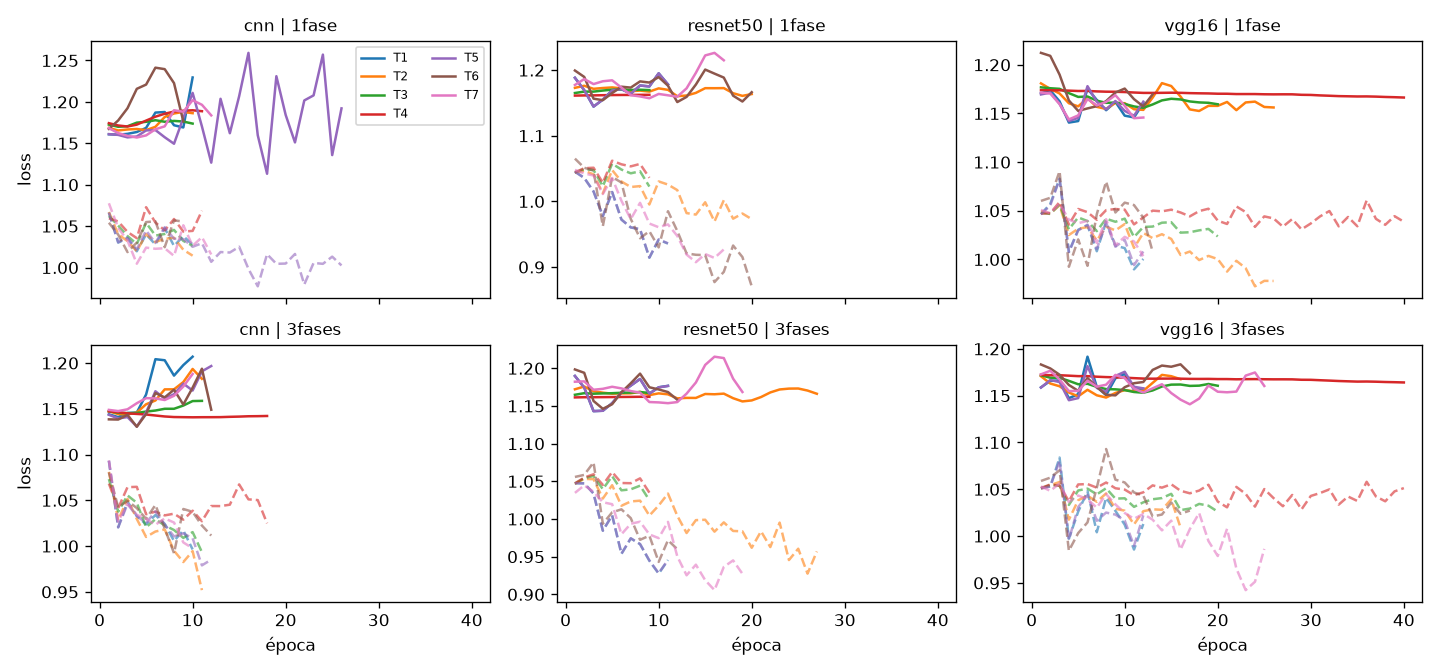
\includegraphics[width=\textwidth]{ajuste_convergencia.png}
\caption{Convergência nas sete tentativas (semente 42): loss de validação em linha cheia e loss de treino
em linha tracejada.}
\label{fig:ajuste}
\end{figure}

Duas ressalvas são necessárias. A loss de validação de uma rede que responde 0,5 para todos é 1,155, e
todas as tentativas ficaram a menos de 0,02 desse valor. Além disso, o desvio padrão da AUC entre
sementes, de até 0,20, é maior do que a diferença entre tentativas. O ajuste não revelou uma configuração
que separe as classes: ele indica que o limite do desempenho não está nesses hiperparâmetros.

\subsection{Treino final}

Com a configuração T5, as três redes foram treinadas nos dois regimes, com o corte central e com todos
os cortes, em 12 modelos. Como os modelos de todos os cortes são avaliados com média e com máximo, há 18
classificadores. A Tabela~\ref{tab:final} traz o resultado no conjunto de teste, de 35 pacientes (12 com
pCR), com o limiar escolhido na validação. O treino levou de 18 a 44 segundos por modelo no corte central
e de 57 a 137 segundos com todos os cortes, cerca de 12 minutos no total.

\begin{table}[ht]
\centering
\caption{Resultados no conjunto de teste com o limiar escolhido na validação. O tempo é o do treino do
modelo; média e máximo usam o mesmo modelo.}
\label{tab:final}
\footnotesize
\setlength{\tabcolsep}{4.5pt}
\begin{tabular}{@{}lllcccccccr@{}}
\toprule
Rede & Regime & Cortes & Limiar & Sens. & Espec. & Prec. & Acur. & F1 & AUC & Tempo (s) \\
\midrule
CNN & 1 fase & central & 0,55 & 0,33 & 0,48 & 0,25 & 0,43 & 0,29 & 0,44 & 19 \\
CNN & 3 fases & central & 0,50 & 0,50 & 0,52 & 0,35 & 0,51 & 0,41 & 0,56 & 18 \\
ResNet50 & 1 fase & central & 0,51 & 0,67 & 0,35 & 0,35 & 0,46 & 0,46 & 0,53 & 19 \\
ResNet50 & 3 fases & central & 0,54 & 0,42 & 0,87 & 0,62 & \textbf{0,71} & 0,50 & \textbf{0,67} & 28 \\
VGG16 & 1 fase & central & 0,51 & 0,42 & 0,65 & 0,38 & 0,57 & 0,40 & 0,49 & 35 \\
VGG16 & 3 fases & central & 0,52 & 0,08 & 0,78 & 0,17 & 0,54 & 0,11 & 0,57 & 44 \\
\midrule
CNN & 1 fase & média & 0,51 & 0,75 & 0,09 & 0,30 & 0,31 & 0,43 & 0,52 & 57 \\
CNN & 3 fases & média & 0,46 & 0,83 & 0,30 & 0,38 & 0,49 & 0,53 & 0,62 & 69 \\
ResNet50 & 1 fase & média & 0,66 & 0,25 & 0,78 & 0,38 & 0,60 & 0,30 & 0,61 & 91 \\
ResNet50 & 3 fases & média & 0,56 & 0,17 & 0,91 & 0,50 & 0,66 & 0,25 & 0,66 & 90 \\
VGG16 & 1 fase & média & 0,49 & 0,33 & 0,78 & 0,44 & 0,63 & 0,38 & 0,63 & 114 \\
VGG16 & 3 fases & média & 0,49 & 0,42 & 0,65 & 0,38 & 0,57 & 0,40 & 0,63 & 137 \\
\midrule
CNN & 1 fase & máximo & 0,52 & 0,25 & 0,52 & 0,21 & 0,43 & 0,23 & 0,33 & 57 \\
CNN & 3 fases & máximo & 0,52 & 0,83 & 0,26 & 0,37 & 0,46 & 0,51 & \textbf{0,67} & 69 \\
ResNet50 & 1 fase & máximo & 0,80 & 0,17 & 0,74 & 0,25 & 0,54 & 0,20 & 0,55 & 91 \\
ResNet50 & 3 fases & máximo & 0,61 & 0,42 & 0,74 & 0,45 & 0,63 & 0,43 & 0,63 & 90 \\
VGG16 & 1 fase & máximo & 0,50 & 0,83 & 0,48 & 0,45 & 0,60 & \textbf{0,59} & 0,61 & 114 \\
VGG16 & 3 fases & máximo & 0,54 & 0,25 & 0,78 & 0,38 & 0,60 & 0,30 & 0,64 & 137 \\
\bottomrule
\end{tabular}
\end{table}

A AUC de teste vai de 0,33 a 0,67. O classificador de maior acurácia e maior AUC é a ResNet50 com três
fases no corte central (acurácia de 0,71 e F1 de 0,50), e o de maior F1 é a VGG16 com uma fase e máximo
dos cortes (0,59). Como referência, responder ``sem pCR'' para todos os pacientes do teste dá acurácia de
0,66: só a ResNet50 de três fases no corte central supera esse valor. Entre as formas de combinar os
cortes, a média teve a maior AUC (0,61 na média dos seis modelos), seguida do máximo (0,57) e do corte
central (0,54).

O limiar tem grande efeito sobre as métricas. Com o limiar fixo em 0,5, a acurácia média dos 18
classificadores é 0,48 e metade deles tem especificidade abaixo de 0,35, porque o peso da classe pCR na
loss desloca as probabilidades para cima. Com o limiar da validação, a acurácia média sobe para 0,54 e
só quatro classificadores ficam abaixo dessa especificidade. O F1 médio cai de 0,48 para 0,37, o que é
esperado: o F1 só olha para a classe positiva e é favorecido por classificar muitos pacientes como pCR.
Os resultados completos com os dois limiares estão no arquivo \texttt{metricas.csv}.

A Figura~\ref{fig:convergencia} mostra a convergência dos modelos treinados com todos os cortes. A loss
de treino cai de forma regular nas redes pré-treinadas, mas a de validação sobe já nas primeiras épocas e
a melhor época é a primeira em três dos seis modelos. A CNN de uma fase é a exceção: sua loss de treino
não sai de 1,05. No corte central o comportamento é o da tentativa T5 da
Figura~\ref{fig:ajuste}, com a melhor época entre a terceira e a quarta nas redes pré-treinadas.

\begin{figure}[ht]
\centering
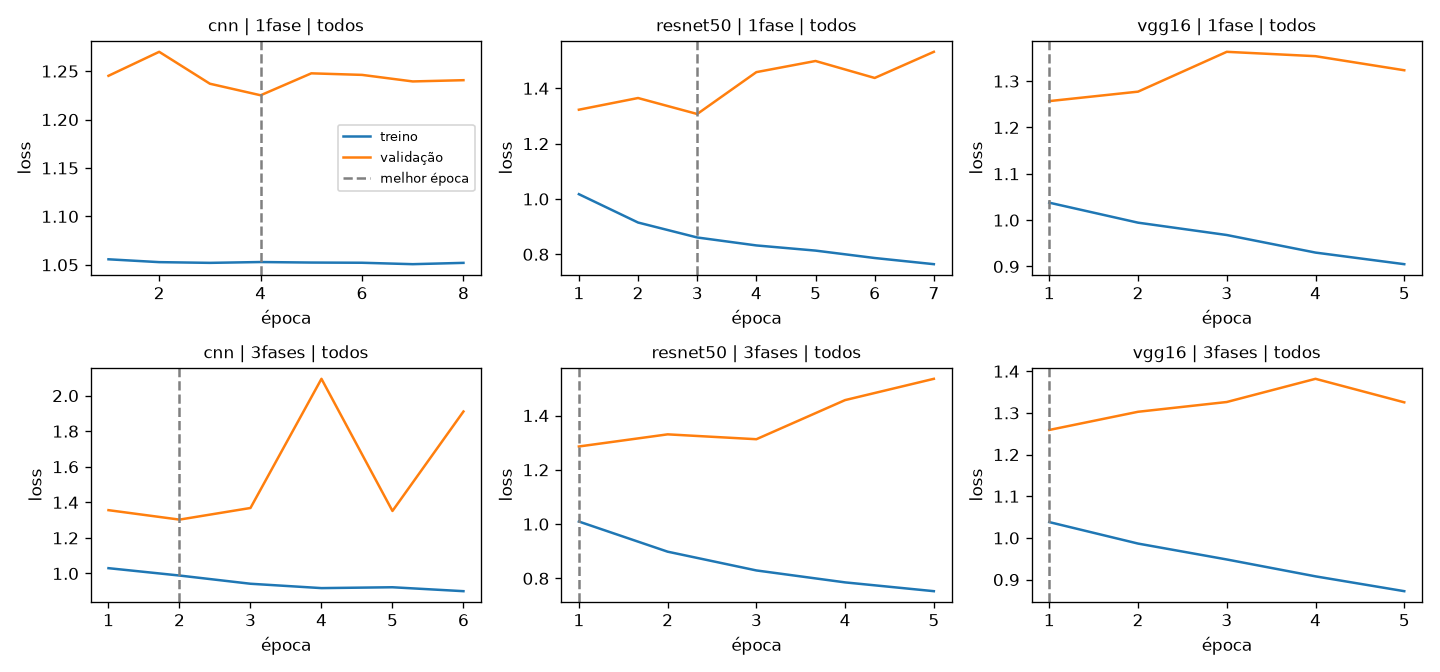
\includegraphics[width=\textwidth]{convergencia_todos.png}
\caption{Loss de treino e de validação no treino final com todos os cortes.}
\label{fig:convergencia}
\end{figure}

\subsection{Exemplos de acertos e erros e Grad-CAM}

A Figura~\ref{fig:gradcam} traz um acerto e um erro da ResNet50 de três fases no corte central. Nos dois
casos a probabilidade fica perto do limiar (0,54 e 0,50) e o mapa de calor se concentra fora do tumor.
Probabilidades pouco separadas são a regra: no corte central, 80\% das saídas de cada rede pré-treinada
no teste cabem em uma faixa de no máximo 0,08 em torno de 0,5. A Tabela~\ref{tab:gradcam} quantifica a
relação entre o mapa e o tumor em todo o conjunto de teste.

\begin{figure}[ht]
\centering
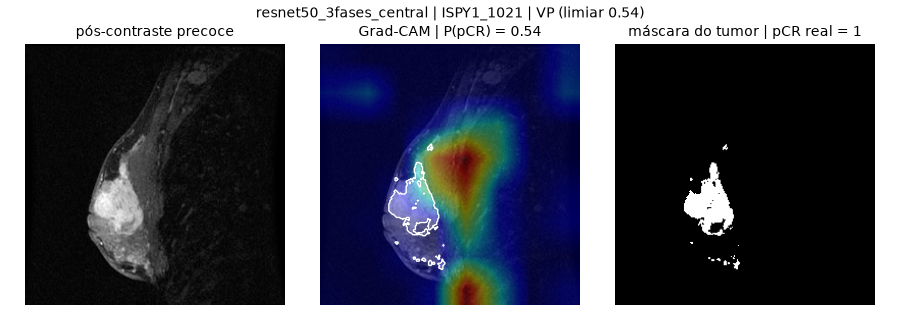
\includegraphics[width=0.76\textwidth]{gradcam_resnet50_3fases_central_VP.png}\\[2pt]
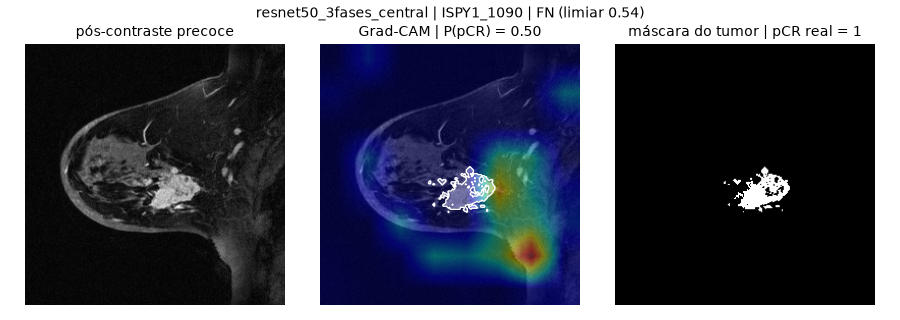
\includegraphics[width=0.76\textwidth]{gradcam_resnet50_3fases_central_FN.png}
\caption{Exemplos da ResNet50 de três fases no corte central: um verdadeiro positivo (acima) e um falso
negativo (abaixo). O contorno branco no painel central é a segmentação do tumor.}
\label{fig:gradcam}
\end{figure}

\begin{table}[ht]
\centering
\caption{Relação entre o Grad-CAM e o tumor no conjunto de teste, nos regimes de uma e de três fases.
``Pico'' é a fração das imagens com o ponto mais quente do mapa dentro do tumor e ``calor'' é a fração
do calor do mapa dentro do tumor. A última coluna é o valor esperado de ``calor'' para um mapa ao acaso.}
\label{tab:gradcam}
\footnotesize
\begin{tabular}{llccccc}
\toprule
 & & \multicolumn{2}{c}{Pico no tumor} & \multicolumn{2}{c}{Calor no tumor} & Área do \\
\cmidrule(lr){3-4}\cmidrule(lr){5-6}
Rede & Treino & 1 fase & 3 fases & 1 fase & 3 fases & tumor \\
\midrule
CNN & corte central & 0\% & 0\% & 0,5\% & 0,1\% & 1,6\% \\
ResNet50 & corte central & 9\% & 3\% & 2,8\% & 2,5\% & 1,6\% \\
VGG16 & corte central & 9\% & 23\% & 3,3\% & 4,7\% & 1,6\% \\
CNN & todos os cortes & 47\% & 15\% & 7,1\% & 6,1\% & 1,2\% \\
ResNet50 & todos os cortes & 1\% & 2\% & 1,2\% & 2,1\% & 1,2\% \\
VGG16 & todos os cortes & 2\% & 5\% & 1,1\% & 2,5\% & 1,2\% \\
\bottomrule
\end{tabular}
\end{table}

\section{Discussão}
\label{sec:discussao}

\subsection{Hiperparâmetros, overfitting, underfitting e convergência}

\textbf{Overfitting.} Com 104 pacientes de treino, o risco dominante é decorar o treino. Seis medidas o
controlam: bases pré-treinadas congeladas, cabeças pequenas (de 2 mil a 33 mil parâmetros), média global
no lugar de camadas totalmente conectadas grandes, \textit{dropout}, decaimento de pesos e aumento de
dados. O \textit{early stopping} é a medida final: ele guarda a época de menor loss de validação. As
curvas mostram que ele atua cedo. No corte central, a loss de treino da ResNet50 cai de 1,05 para 0,94 em
11 épocas enquanto a de validação sobe a partir da terceira. Com todos os cortes, a rede vê 25 vezes mais
imagens por época, mas elas vêm dos mesmos 104 pacientes, e a validação piora ainda antes.

\textbf{Underfitting.} Ocorreu em dois casos. Com taxa de aprendizado de $10^{-5}$, 40 épocas não bastam
para mover a loss de treino. E a CNN própria de uma fase, treinada com todos os cortes e decaimento de
$10^{-2}$, ficou com loss de treino constante em 1,05 e saídas entre 0,50 e 0,52 para todos os pacientes,
o que indica que a regularização que ajudou no corte central foi forte demais nesse caso.

\textbf{Velocidade de convergência.} A taxa de $10^{-3}$ leva as redes pré-treinadas à melhor época em
3 ou 4 passagens pelo treino no corte central e em 1 a 3 com todos os cortes. Com a paciência de 8 e de 4
épocas, nenhum treino passou de 26 épocas, o que explica os tempos de segundos a poucos minutos.

\textbf{Demais hiperparâmetros.} O tamanho do lote e o \textit{dropout} não alteraram a validação além do
ruído (T6 e T7). O limiar escolhido na validação corrige a tendência a prever pCR criada pelo peso das
classes, mas é estimado com 33 pacientes e por isso é instável: variou de 0,46 a 0,80 entre os modelos.

\subsection{Respostas às perguntas do trabalho}

\textbf{As três fases produzem resultados melhores que uma fase?} No treino final, a AUC de teste com
três fases foi maior nos nove pares comparados (mesma rede e mesma combinação de cortes), com média de
0,63 contra 0,52. Essa tendência, porém, não permite confirmar a hipótese. O erro padrão da AUC com 35
pacientes de teste é de cerca de 0,10, igual à diferença observada. Nos 63 pares do ajuste, com três
sementes, a diferença média caiu para 0,02 no teste e foi de $-0{,}02$ na validação. Além disso, os nove
pares usam os mesmos pacientes de teste e não são independentes. A conclusão é que os dados não mostram
prejuízo no uso das três fases e sugerem um ganho pequeno, que só um conjunto maior poderia confirmar.

\textbf{Qual rede teve melhor desempenho?} Na média de seus seis classificadores, a ResNet50 teve
acurácia de 0,60 e AUC de 0,61, a VGG16 0,59 e 0,59, e a CNN própria 0,44 e 0,52. As duas redes
pré-treinadas ficaram equivalentes e acima da CNN própria, que tem de aprender todos os filtros com
poucos dados. O melhor classificador isolado foi a ResNet50 de três fases no corte central, mas o
intervalo de confiança de 95\% da sua AUC, de aproximadamente 0,47 a 0,87, inclui o acaso.

\textbf{Quais erros são mais frequentes?} Depende do limiar. Com o limiar fixo em 0,5 predominam os
falsos positivos: 65\% dos pacientes sem pCR são classificados como pCR, contra 27\% de falsos negativos
entre os pacientes com pCR. Com o limiar da validação os erros se equilibram em número (168 falsos
positivos e 121 falsos negativos nos 18 classificadores), mas a taxa de falsos negativos passa a ser a
maior: 56\% dos pacientes com pCR deixam de ser identificados, contra 41\% de falsos positivos.

\textbf{O Grad-CAM destaca as regiões tumorais?} Em geral, não. Nas redes pré-treinadas, o ponto mais
quente do mapa cai dentro do tumor em no máximo 23\% das imagens e a fração de calor dentro do tumor
fica entre 1 e 3 vezes a esperada ao acaso (Tabela~\ref{tab:gradcam}). A CNN do corte central olha para
fora da lesão. A exceção é a CNN treinada com todos os cortes, cujo mapa concentra no tumor de 5 a 6
vezes mais calor que o acaso, sem que isso se traduza em melhor classificação. Parte do resultado se deve
à resolução do mapa: na ResNet50 ele tem $8 \times 8$ células, cada uma maior do que muitos tumores.

\textbf{Quais as principais limitações?} (i) O conjunto é pequeno: 104 pacientes de treino, 33 de
validação e 35 de teste tornam instáveis o ajuste, o limiar e a comparação entre modelos. (ii) O tumor
ocupa cerca de 2\% da imagem de entrada, e as redes não recebem indicação de onde ele está; usar a
máscara como canal ou recortar a imagem na lesão é o próximo passo natural. (iii) As bases congeladas
foram treinadas em fotografias e não foram adaptadas à ressonância. (iv) As estratégias avaliadas tratam
cada corte isoladamente e não usam a informação tridimensional. (v) O treino final usou uma única
semente. (vi) Dados clínicos como o subtipo molecular, sabidamente ligados à pCR, não foram usados por
exigência do enunciado.

\section{Conclusão}

O sistema desenvolvido cumpre as funções propostas: visualização dos volumes com a segmentação, aumento
de dados, treino de três redes em dois regimes, três formas de combinar cortes e classificação com
Grad-CAM. Os classificadores, porém, ficaram próximos do acaso, e o ajuste de hiperparâmetros mostrou que
o limite não está na configuração do treino, mas na quantidade de dados e na forma de apresentar o tumor
à rede. O uso das três fases mostrou tendência de ganho no teste, sem significância estatística.

\begin{thebibliography}{99}

\bibitem[Deng et al. 2009]{deng2009}
Deng, J., Dong, W., Socher, R., Li, L.-J., Li, K. e Fei-Fei, L. (2009).
\newblock ImageNet: A large-scale hierarchical image database.
\newblock In {\em IEEE Conference on Computer Vision and Pattern Recognition}, p. 248--255.

\bibitem[Fridman et al. 2026]{fridman2026}
Fridman, N. et al. (2026).
\newblock BreastDCEDL: A standardized deep learning-ready breast DCE-MRI dataset of 2,070 patients.
\newblock {\em Scientific Data}, 13(1):264.

\bibitem[He et al. 2016]{he2016}
He, K., Zhang, X., Ren, S. e Sun, J. (2016).
\newblock Deep residual learning for image recognition.
\newblock In {\em IEEE Conference on Computer Vision and Pattern Recognition}, p. 770--778.

\bibitem[Hylton et al. 2012]{hylton2012}
Hylton, N. M. et al. (2012).
\newblock Locally advanced breast cancer: MR imaging for prediction of response to neoadjuvant
  chemotherapy -- results from ACRIN 6657/I-SPY TRIAL.
\newblock {\em Radiology}, 263(3):663--672.

\bibitem[Ioffe e Szegedy 2015]{ioffe2015}
Ioffe, S. e Szegedy, C. (2015).
\newblock Batch normalization: Accelerating deep network training by reducing internal covariate shift.
\newblock In {\em International Conference on Machine Learning}, p. 448--456.

\bibitem[Kingma e Ba 2015]{kingma2015}
Kingma, D. P. e Ba, J. (2015).
\newblock Adam: A method for stochastic optimization.
\newblock In {\em International Conference on Learning Representations}.

\bibitem[Paszke et al. 2019]{paszke2019}
Paszke, A. et al. (2019).
\newblock PyTorch: An imperative style, high-performance deep learning library.
\newblock In {\em Advances in Neural Information Processing Systems 32}, p. 8024--8035.

\bibitem[Selvaraju et al. 2017]{selvaraju2017}
Selvaraju, R. R., Cogswell, M., Das, A., Vedantam, R., Parikh, D. e Batra, D. (2017).
\newblock Grad-CAM: Visual explanations from deep networks via gradient-based localization.
\newblock In {\em IEEE International Conference on Computer Vision}, p. 618--626.

\bibitem[Simonyan e Zisserman 2015]{simonyan2015}
Simonyan, K. e Zisserman, A. (2015).
\newblock Very deep convolutional networks for large-scale image recognition.
\newblock In {\em International Conference on Learning Representations}.

\bibitem[Srivastava et al. 2014]{srivastava2014}
Srivastava, N., Hinton, G., Krizhevsky, A., Sutskever, I. e Salakhutdinov, R. (2014).
\newblock Dropout: A simple way to prevent neural networks from overfitting.
\newblock {\em Journal of Machine Learning Research}, 15:1929--1958.

\bibitem[Youden 1950]{youden1950}
Youden, W. J. (1950).
\newblock Index for rating diagnostic tests.
\newblock {\em Cancer}, 3(1):32--35.

\end{thebibliography}

\end{document}
